% ================================================================= 10
\section{Evaluation setup}\label{sec:eval}

\paragraph{Benchmarks} \textbf{LongMemEval-S}~\cite{longmemeval}: 82 questions (12 per question type plus 10
abstentions, fixed seed), each over a chat history of about 48 sessions and 115k tokens. \textbf{BEAM}~\cite{beam}: its 20
shortest 100K conversations, with the two abilities a write-time policy serves, \emph{contradiction resolution} and
\emph{knowledge update}, two questions each per conversation (80 in all), scored by BEAM's rubric judge.
\textbf{OrgProbe}: 17 questions of our own over a fictional company's scope tree (Section~\ref{sec:orgprobe}).

\paragraph{Systems} \textbf{\mx{}} in \textbf{ranked} recall (4,000-token budget) and \textbf{full} memory (everything
visible). \textbf{mem0} open source (\code{mem0ai} 2.2.1, default prompts, \code{top\_k}=30). \textbf{Zep}: Graphiti
0.31.2 on FalkorDB with its combined hybrid search, with its default LLM judge or with Graphiti's own \code{JevClient}.
Two baselines: \textbf{full context} (every session given to the answering model) and \textbf{chunk RAG} (chunks of
800--1,000 tokens, most similar first, same 4,000-token budget).

\paragraph{Held equal} Within each comparison every system used the same extraction model, embeddings
(\code{text-embedding-3-small}), answering model and prompt (temperature 0) and judge (Claude Sonnet 5.5 with the
benchmark's own prompts). LongMemEval and the Zep comparison extracted with Claude Haiku 5.5 and answered with Haiku
4.5; BEAM used Haiku 5.5 for both; OrgProbe used Haiku 4.5 for both. Every session was inserted at its
own date. The other systems ran with documented defaults. LongMemEval comparisons are paired on question (exact
McNemar); BEAM uses bootstrap intervals and a paired sign test.

% ================================================================= 11a
\section{Memory efficiency against mem0}\label{sec:efficiency}

\begin{figure}[!htb]
\centering
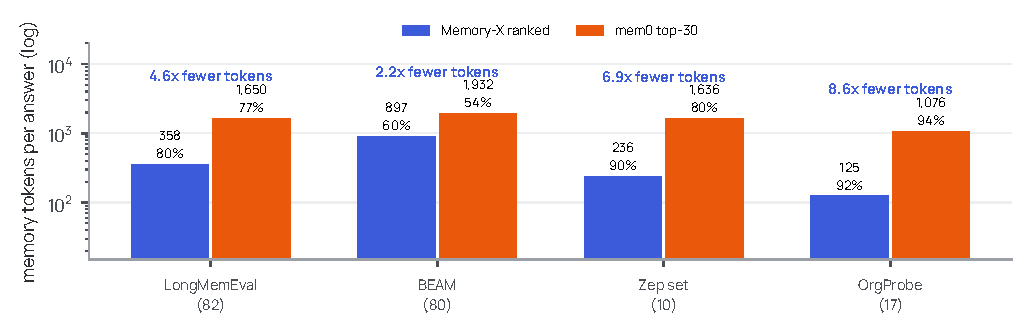
\includegraphics[width=\linewidth]{figures/fig_efficiency.pdf}
\caption{\textbf{Memory tokens given to the answering model per question}, \mx{} ranked recall against mem0 top-30, with
each system's score above its bar (log scale).}
\label{fig:efficiency}
\end{figure}

On every benchmark \mx{} hands the answering model 2 to 9 times fewer memory tokens than mem0, at higher accuracy on
LongMemEval, BEAM and the Zep set and within one question on OrgProbe (Figure~\ref{fig:efficiency}), for about the
same ingest cost. Every token in that block is paid for on every question an agent asks; the sections below give the
detail.

% ================================================================= 11
\section{Results on LongMemEval}\label{sec:lme}

\begin{table}[!htb]
\centering\small
\setlength{\tabcolsep}{4pt}
\begin{tabular}{@{}l c r r r r@{}}
\toprule
\thead{System} & \thead{Accuracy (95\% CI)} & \thead{vs mem0 (paired)} & \thead{Memory tokens} & \thead{Recall p50} & \thead{Evidence recall}\\
\midrule
\mx{} full memory & \best{89.0\%} [80, 94] & 12 / 2, $p=0.013$ & 24,464 & 631 ms & 0.99\\ \rowrule
\mx{} ranked (4k) & 80.5\% [71, 88] & 12 / 9, $p=0.66$ & \best{358} & 650 ms & 0.89\\ \rowrule
mem0 top-30 & 76.8\% [67, 85] & -- & 1,650 & 689 ms & 0.91\\ \rowrule
chunk RAG (4k) & 73.2\% [63, 82] & 11 / 14, $p=0.69$ & 3,968 & -- & 0.91\\ \rowrule
full context & 68.3\% [58, 77] & 10 / 17, $p=0.25$ & 117,009 & -- & \best{1.00}\\
\bottomrule
\end{tabular}
\caption{\textbf{LongMemEval-S, 82 questions.} \mx{} and mem0 ingested every history fresh with Haiku 5.5; all systems
answered with Haiku 4.5 and were judged by Sonnet 5.5. ``vs mem0'': questions only this system / only mem0 got right,
exact McNemar. Memory tokens: mean block given to the answering model. Evidence recall: share of gold evidence sessions
represented in that block.}
\label{tab:lme}
\end{table}

\begin{figure}[!htb]
\centering
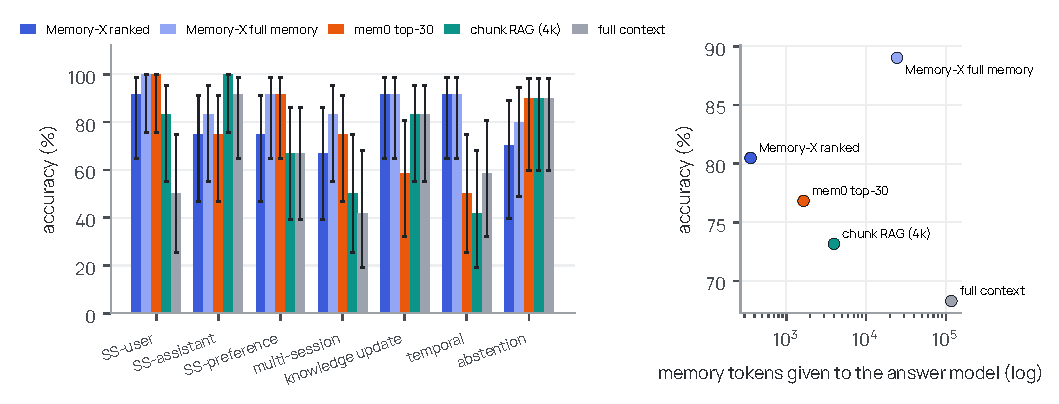
\includegraphics[width=\linewidth]{figures/fig_lme.pdf}
\caption{\textbf{Accuracy by question type} (left, Wilson 95\% intervals) and \textbf{against memory-block size}
(right, log scale).}
\label{fig:lme}
\end{figure}

\mx{} ranked recall answered 80.5\% of questions from a 358-token block, \textbf{4.6 times smaller} than mem0's 1,650
tokens, against mem0's 76.8\% (12 to 9, not significant). With its full memory \mx{} reached 89.0\%, significantly
above mem0 (12 to 2, $p=0.013$), chunk retrieval (17 to 4, $p=0.007$) and full context (20 to 3, $p<0.001$). The
largest per-type gaps are on temporal reasoning (11 of 12 against mem0's 6) and knowledge updates (11 against 7), where
\mx{}'s dated related facts and replaced-version history let the answering model pick the newer value. Ranked recall
keeps 1.5\% of the full memory's tokens; the gap to full memory (1 to 8, $p=0.04$) is spread across question types,
mostly facts the grader judged background that the answer needed.

\begin{figure}[!htb]
\centering
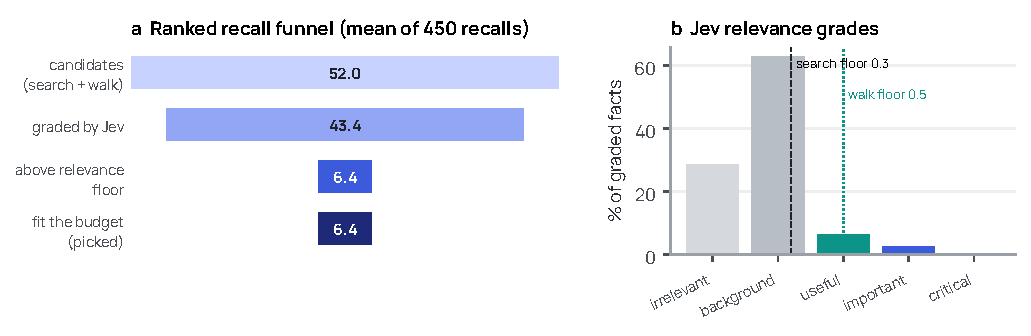
\includegraphics[width=\linewidth]{figures/fig_recall.pdf}
\caption{\textbf{What ranked recall does with its candidates} on LongMemEval. (a) Mean facts per step. (b) Jev's
relevance grade for every graded fact.}
\label{fig:recall}
\end{figure}

\paragraph{Where the small block comes from} One Jev request grades about 43 candidates per question; 90\% are graded
\emph{irrelevant} or \emph{background} and cut, leaving about 6 facts (Figure~\ref{fig:recall}).

\paragraph{Ingest cost} With the cost cuts of Section~\ref{sec:arch}, \mx{} ingest cost \$0.142 per history (extraction
\$0.055, Jev \$0.087) against about \$0.13 for mem0, storing 552 facts per history. Before the cuts the same histories
cost \$0.214 and produced 811 facts, with no loss of accuracy on a 10-question check (8 and 9 of 10 correct,
Table~\ref{tab:extractcost}).

\begin{table}[!htb]
\centering\small
\begin{tabular}{@{}l r r r r r@{}}
\toprule
\thead{Per history, Haiku 5.5} & \thead{Facts} & \thead{Output tokens} & \thead{Extraction} & \thead{Jev} & \thead{Total}\\
\midrule
before the cuts & 811 & 113k & \$0.100 & \$0.114 & \$0.214\\ \rowrule
after the cuts & \best{552} & \best{63k} & \best{\$0.055} & \best{\$0.087} & \best{\$0.142}\\ \rowrule
mem0 (reference) & & & & & \$0.13\\
\bottomrule
\end{tabular}
\caption{\textbf{Extraction cost.} The cuts: an assistant's list as one fact, a slimmer output schema, continuation
instead of re-extraction, a cached prompt prefix and the chit-chat gate. Measured from per-ingest receipts (cache reads at the cache-read price) and metered
Jev cost. The chit-chat gate rarely fires on LongMemEval (about one turn per history). Batch extraction for queued
inserts halves the extraction price again; it is not used in the benchmarks.}
\label{tab:extractcost}
\end{table}


% ================================================================= 11b
\section{Results on BEAM}\label{sec:beam}

\begin{table}[!htb]
\centering\small
\setlength{\tabcolsep}{4pt}
\begin{tabular}{@{}l c c c r r@{}}
\toprule
\thead{System} & \theadm{Contra-\\diction (40)} & \theadm{Update\\(40)} & \theadm{Both (80)\\95\% CI} & \theadm{\mx{} wins\\/ losses} & \theadm{Memory\\tokens}\\
\midrule
\mx{} ranked (4k) & \best{66.2} & 53.8 & \best{60.0} [51, 68] & -- & \best{897}\\ \rowrule
mem0 top-30 & 55.6 & 51.9 & 53.8 [45, 62] & 29 / 15, $p=0.049$ & 1,932\\ \rowrule
full context & 46.6 & \best{61.3} & 53.9 [45, 63] & 27 / 14, $p=0.06$ & 175,931\\ \rowrule
chunk RAG (4k) & 45.9 & 45.6 & 45.8 [37, 54] & 35 / 14, $p=0.004$ & 3,958\\
\bottomrule
\end{tabular}
\caption{\textbf{BEAM-100K, 20 conversations, 80 questions; BEAM's rubric judge (\%).} Haiku 5.5 extraction and
answering. Bootstrap 95\% intervals; wins / losses count questions where \mx{} scored higher / lower (two-sided sign
test).}
\label{tab:beam}
\end{table}

\begin{figure}[!htb]
\centering
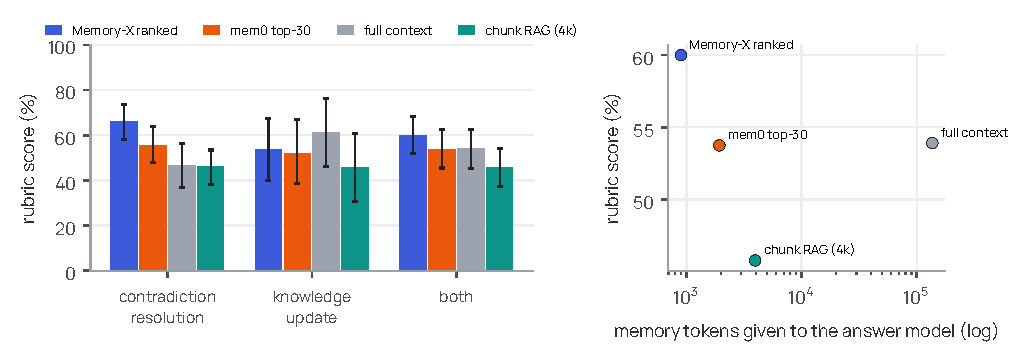
\includegraphics[width=\linewidth]{figures/fig_beam.pdf}
\caption{\textbf{BEAM rubric score by ability} (left, bootstrap 95\% intervals) and \textbf{against the size of the
memory block} (right, log scale).}
\label{fig:beam}
\end{figure}

\mx{} scored highest overall (60.0\%) with the smallest block: \textbf{897 tokens, 2.2 times fewer than mem0} (53.8\%)
and 196 times fewer than full context (53.9\%). Against mem0 it won 29 questions and lost 15 ($p=0.049$). The gain is
in \textbf{contradiction resolution}: 66.2\% against 55.6\% (22 wins, 9 losses, $p=0.029$). These questions reward
naming both sides of a conflict. Because a replacement needs $P\ge0.9$, an incompatible pair Jev is unsure about stays
as two related, dated facts, and the answering model sees both: 28 of \mx{}'s 40 answers flagged the contradiction,
against 20 for mem0 and 20 for full context. On \textbf{knowledge updates} \mx{} and mem0 were level (53.8\% and
51.9\%), and full context did best (61.3\%).

Ingesting the 20 conversations cost \mx{} \$0.136 per conversation (extraction \$0.053, Jev \$0.083). In mem0, 97
extraction responses could not be parsed and stored nothing; we left that behaviour as shipped.


% ================================================================= 11c
\section{Comparison with Zep}\label{sec:zep}

Graphiti's ingest makes several LLM calls per episode (about 6.9 million input tokens for one 115k-token history), so we
ran it on 10 LongMemEval questions, two per type, with every system ingesting on Haiku 5.5. The set was chosen around
questions \mx{} had missed in an earlier version, so it is not random and the differences are descriptive.

\begin{table}[!htb]
\centering\small
\setlength{\tabcolsep}{4pt}
\begin{tabular}{@{}l c r r r@{}}
\toprule
\thead{System} & \theadm{Correct\\/ 10} & \theadm{Memory\\tokens} & \theadm{Ingest\\\$ / question} & \theadm{LLM calls\\/ question}\\
\midrule
\mx{} ranked (4k) & \best{9} & \best{236} & 0.135 & 81 + 1,162 Jev\\ \rowrule
\mx{} full memory & \best{9} & 23,989 & 0.135 & 81 + 1,162 Jev\\ \rowrule
mem0 top-30 & 8 & 1,636 & \best{0.131} & 49\\ \rowrule
Zep + Jev & 6 & 2,369 & 0.60 & 153 + 381 Jev\\ \rowrule
Zep (LLM judge) & 5 & 2,311 & 0.71 & 452\\
\bottomrule
\end{tabular}
\caption{\textbf{10 LongMemEval questions, Haiku 5.5 extraction.} Ingest cost is metered per call. Jev requests cost
about \$0.00007 each.}
\label{tab:zep}
\end{table}

\begin{figure}[!htb]
\centering
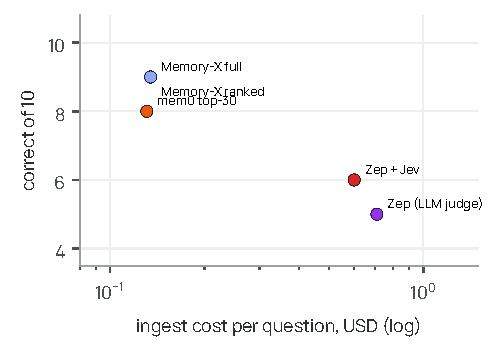
\includegraphics[width=0.55\linewidth]{figures/fig_zep.pdf}
\caption{\textbf{Correct answers against ingest cost} (log scale).}
\label{fig:zep}
\end{figure}

\mx{} answered 9 of 10 with ranked recall, against mem0's 8, with \textbf{6.9 times fewer memory tokens} and the same
ingest cost. Zep answered 5 with its LLM judge and 6 with Jev, at four to five times \mx{}'s ingest cost and with
blocks ten times larger. Routing Graphiti's judgement calls to Jev cut its cost by about a sixth. Graphiti asks two binary questions at
fixed thresholds and invalidates edges graph-wide; \mx{} asks a five-way question with per-outcome floors, guards and
scope-local corrections.


% ================================================================= 12
\section{Organisational probe}\label{sec:orgprobe}

LongMemEval has no scopes, few named colleagues and nothing that tries to steer the memory. OrgProbe
(\code{eval/orgprobe}) covers those: a company handbook at \code{memory.acme}, a reseller note with a planted instruction
aimed at AI systems, an SRE notice that changes the escalation channel for \code{memory.acme.sre} only, five
conversations with an engineer over six weeks, and 16 filler sessions so that memory (about 300 facts) exceeds the
budget. Seventeen questions test entity hops, name variants (``Priya'', ``K8s''), updates, scope-specific answers and the
planted instruction; each is answered three times. mem0 maps each scope to a \code{user\_id} and searches every
ancestor.

\begin{table}[!htb]
\centering\small
\setlength{\tabcolsep}{4pt}
\begin{tabular}{@{}l c c c c c c r@{}}
\toprule
\thead{System} & \thead{Hop (6)} & \thead{Variant (3)} & \thead{Update (3)} & \thead{Scope (2)} & \thead{Injection (3)} & \thead{All (17)} & \thead{Tokens}\\
\midrule
\mx{} ranked (2k) & \best{6.0} & \best{3.0} & 2.0 & \best{2.0} & 2.7 & 15.7 & 125\\ \rowrule
\mx{} ranked, no walk & 5.0 & \best{3.0} & \best{3.0} & \best{2.0} & \best{3.0} & \best{16.0} & \best{73}\\ \rowrule
\mx{} full memory & \best{6.0} & \best{3.0} & 2.0 & \best{2.0} & \best{3.0} & \best{16.0} & 10,779\\ \rowrule
mem0 top-30 & 5.0 & \best{3.0} & \best{3.0} & \best{2.0} & \best{3.0} & \best{16.0} & 1,076\\ \rowrule
mem0 top-10 & 3.7 & \best{3.0} & \best{3.0} & \best{2.0} & \best{3.0} & 14.7 & 347\\
\bottomrule
\end{tabular}
\caption{\textbf{OrgProbe}, questions answered correctly (mean of three answers). Tokens: mean memory block. No system
leaked the planted password or vendor. Haiku 4.5 extraction and answering for both systems.}
\label{tab:orgprobe}
\end{table}

\mx{} answered 15.7 of 17 from a 125-token block, \textbf{8.6 times fewer tokens} than mem0's top-30 (16 of 17); cut
to top-10 (347 tokens), mem0 lost hop questions. The scope question is now answered correctly: the SRE notice is
stored as one fact (``the SRE team's channel changed from \#ops-alerts to \#sre-pager''), as the extraction rule
intends. \mx{}'s update miss is a known gap: ``the user moved to Lisbon'' and ``Alex lives in Porto'' name the same
person differently, so reconcile judged them only related (0.42) and the answering model chose Porto; a per-scope
subject name for ``the user'' would link them. Both extractors dropped the planted instruction, so the injection check
was tested directly (Section~\ref{sec:decisions}).


% ================================================================= 12b
\section{Multi-hop recall: HopProbe}\label{sec:hop}

LongMemEval and OrgProbe questions share words with the facts that answer them, so search finds those facts and the
walk has nothing to add. HopProbe (\code{eval/hopprobe}) isolates the case the walk is for: 44 questions whose answer
fact shares no content word with the question and is reachable only through a bridge fact. ``In which town is the
person responsible for Orion based?'' needs ``Orion is owned by Ingrid Halvorsen'' and then ``Ingrid Halvorsen lives in
Trondheim''; every answer fact has look-alikes about other people (``Kofi Mensah lives in Accra''), so search returns a
pile of candidates it cannot tell apart. The directory sits among 16 filler chat sessions (228 facts in all); answers are
scored exactly (the expected value and no look-alike value), with no judge.

\begin{table}[!htb]
\centering\small
\begin{tabular}{@{}l c c c@{}}
\toprule
\thead{Ranked recall (2k)} & \thead{Correct / 44} & \thead{Answer fact in the block} & \thead{Memory tokens}\\
\midrule
walk on & \best{41} & 42 & 113\\ \rowrule
walk off & 28 & 28 & 103\\
\bottomrule
\end{tabular}
\caption{\textbf{HopProbe}, same stored memory, Haiku 4.5 answering. Paired: 14 questions only with the walk, 1 only
without, exact McNemar $p=0.001$.}
\label{tab:hop}
\end{table}

With the walk, 41 of 44 answers were right; without it, 28 (14 to 1, $p=0.001$), at about the same block size. Every miss
without the walk is the same failure: the block holds the bridge (``Vega is owned by Mei Tanaka'') but not the answer,
and the model says it does not know. The walk follows the shared entity, and joint grading keeps the reached fact
because it is judged together with its bridge. On LongMemEval the walk changes nothing (80.5\% with and without), so its
cost is one bounded graph query when it does not help.


% ================================================================= 13
\section{Decision quality}\label{sec:decisions}

The benchmark runs logged 415,106 Jev decisions. Median request latency was 166--178\,ms for insert steps and
254\,ms for a recall grade carrying up to 48 questions (Figure~\ref{fig:latency}).

\subsection{Why destructive verdicts need 0.9}

Without human labels, we asked Claude Sonnet 5.5 the same questions with the same definitions and context, on samples
stratified by Jev's probability: 240 reconcile verdicts, 196 destructive verdicts (same, replaces, covers) and 154 entity
decisions (Figure~\ref{fig:calibration}). Agreement with a larger model is not correctness, but it should rise with Jev's
probability if thresholds are meaningful.

\begin{figure}[!htb]
\centering
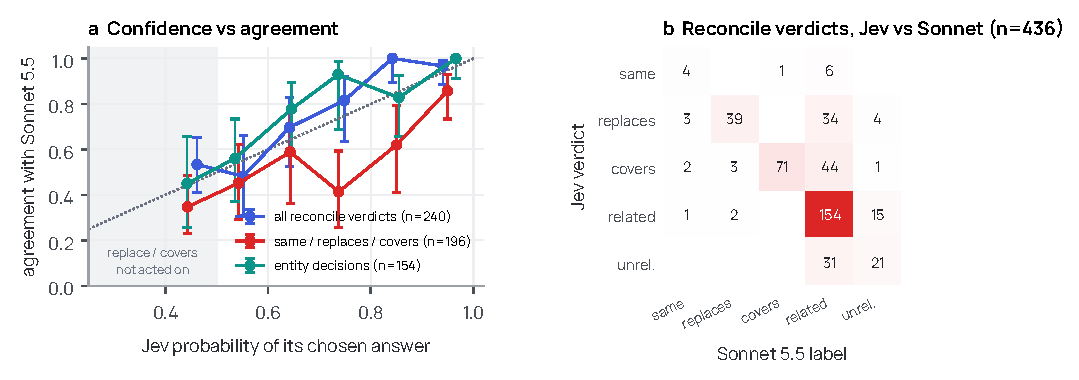
\includegraphics[width=\linewidth]{figures/fig_calibration.pdf}
\caption{\textbf{Jev's confidence against agreement with a larger model.} (a) Agreement with Claude Sonnet 5.5 by Jev's
probability bin, with Wilson intervals; the dotted line is perfect agreement-calibration. Samples are stratified by
probability, so pooled rates are not population rates. (b) Jev's reconcile verdict against Sonnet's label over both
verdict samples.}
\label{fig:calibration}
\end{figure}

Overall, agreement rises with probability and sits near the diagonal (about 0.5 below 0.6, 0.97--1.0 above 0.9).
Destructive verdicts are the exception: agreement stays between 0.41 and 0.62 from 0.5 to 0.9 and reaches 0.86 only
above 0.9, and when Sonnet disagreed it almost always said \emph{related}. An option-order check pointed the same way:
shuffling the five options changed 5 of 30 destructive labels below 0.9 and none of 8 above. Hence the 0.9 floor on
``replaces'' and ``covers''. A narrower follow-up question for the band below the floor (``can both statements be true
at once?'') did not help: on 67 labelled verdicts between 0.6 and 0.9 Jev answered ``yes'' (median 0.96) whether or
not the reference agreed with the replacement, so it is off by default. Entity decisions tracked their probability closely (0.93 agreement at the 0.7 merge
threshold), and nearly all similar-embedding pairs were judged different, as the asymmetric prior intends.

\subsection{The injection check, tested directly}

In OrgProbe both extractors dropped the planted instruction, so we sent 12 planted instructions and 12 ordinary statements
that merely sound imperative (``The user asked the assistant to always include sources'', ``Production deploys require
two approvals'') straight to the sort request. All 12 planted instructions scored at least 0.75 (ten at 0.93 or more,
so they would be rejected outright; two would be stored flagged and kept out of recall). The 12 ordinary statements
scored 0.03--0.42; two user preferences about the assistant's behaviour came closest to the 0.5 flag (0.41 and 0.42).
The probe is author-written and small; it shows the check separates obvious cases with margin, not that it resists
adaptive attacks, against which Jev's own documentation warns~\cite{typesafe}.

